\documentclass[aspectratio=1610, 13pt]{beamer}
\usepackage{verbatim}
\usepackage{amsmath}
\usepackage{amsthm}
\usepackage{multicol}
\usepackage{graphics}
\usepackage{color}
\usepackage{stmaryrd}\usefonttheme[onlymath]{serif}

\title{Progess Report 2}
\date{\today}
\author{Presentor: Xie Li}
\begin{document}
\maketitle

\begin{frame}\frametitle{Overview}
\begin{itemize}
\item Running SV-COMP cases on SMACK.
\item Memory model and its construction.
\item Insert assertion to Boogie.
\end{itemize}
\end{frame}

\begin{frame}\frametitle{}

\end{frame}


\begin{frame}\frametitle{Memory Model and Region: DSA}

Each DS node represent a set of dynamic memory object (may be infinite), different nodes represent disjoint sets of objects.

\begin{definition}[Data Structure Graph]
A DS graph for a function $F$ is $G(F) = \langle N, E, E_V, N_{call}\rangle$.
\begin{itemize}
\item $N$ is a set of nodes.
\item $E$ is a set of edges in the graph, $E$ is a function of the type $\langle n_s, f_s\rangle \rightarrow \langle n_d, f_d\rangle$, where $n_s, n_d \in N$ and $f_s\in field(T(n_s)), f_d\in field(T(n_d))$.

This node-field pair is called a \emph{cell}, non-pointer compatible and register variables are mapped to $\langle null, 0\rangle$

$E$ is a function.
\item $E_V$ is a partial function for pointer-compatible variables in $vars(f)$. i.e. $vars(f) \rightarrow \langle
n, f\rangle$.

\item $N_{call}$ is the set of call nodes which is a subset of $N$. Every call node is a tuple of node-field pairs: $\langle r, f, a_1, \ldots, a_k\rangle$. Each element can also be regarded as a points-to edge in the graph.

\end{itemize}
\end{definition}

\end{frame}

\begin{frame}\frametitle{Visualization of DSG}
\begin{center}
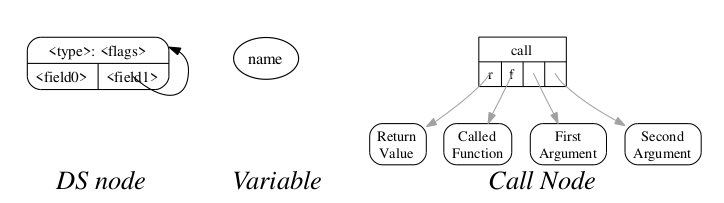
\includegraphics[scale=0.50]{dsg_legend.png}
\end{center}
\end{frame}

\begin{frame}\frametitle{Visualization of DSG}

\begin{center}
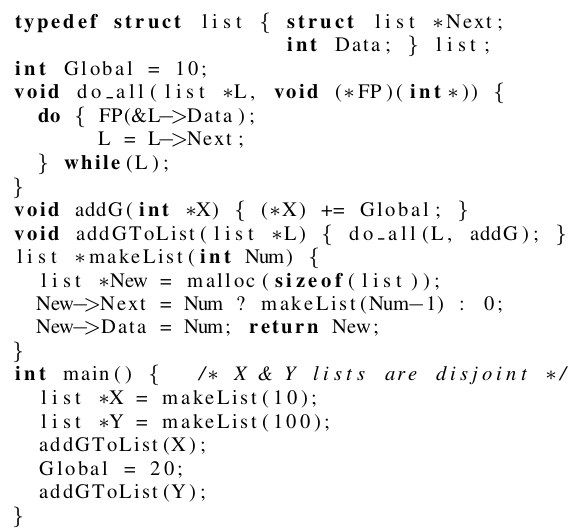
\includegraphics[scale=0.3]{code.png}

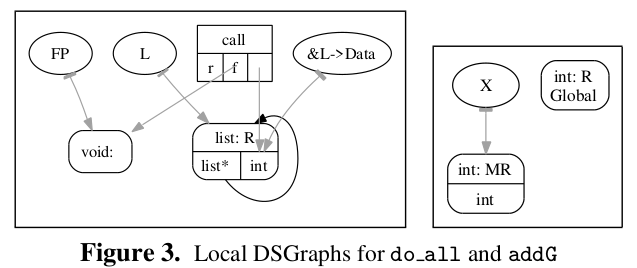
\includegraphics[scale=0.4]{doall.png}
\end{center}
\end{frame}

\begin{frame}\frametitle{Graph Node and Field}
\begin{center}
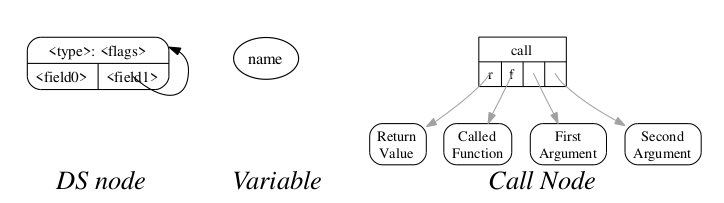
\includegraphics[scale=0.4]{dsg_legend.png}
\end{center}
There are three pieces of information of a DS Node $n$.
\begin{itemize}
\item $T(n)$.
\item $G(n)$ is a set of global objects represented by $n$.
\item $flag(n)\subseteq \{\mathbf{H,S,G,U,A,M,R,C,O}\}$
\end{itemize}
\end{frame}

\begin{frame}\frametitle{Meaning of the Flags}
\begin{itemize}
\item Storage class flags: \textbf{H}eap, \textbf{S}tack, \textbf{G}lobal, \textbf{U}nknown.

\item Whether a memory object is loaded or stored: \textbf{R}eferenced, \textbf{M}odified.

\item \textbf{C}omplete.
\item C\textbf{O}llapsed: nodes representing multiple, incompatible types of objects: type homogenous, \emph{use} of a object.
\item \textbf{A}rray flag.
\end{itemize}

\end{frame}

\begin{frame}\frametitle{Construction of the DSG}
Three steps:
\begin{itemize}
\item Construct the DSG for each function.
\item Bottom-up analysis.
\item Top-down analysis.

\end{itemize}
Two important properties:
\begin{itemize}
\item 
\item 
\end{itemize}
\end{frame}

\begin{frame}\frametitle{Primitive Graph Operation}

\end{frame}

\begin{frame}\frametitle{Insert Self-defined Assertion}

\end{frame}



\end{document}